\documentclass[10pt,letterpaper]{article}
\usepackage{tools}
\usepackage{enumitem}
%\settextfont{B Nazanin}
\usepackage{lipsum}
\setlength{\parskip}{3mm}
\setlength{\parindent}{0mm}
\newcommand{\wid}{0.49\textwidth}
\newcommand{\widone}{60mm}
\begin{document}
\Large
\begin{center}
In the name of beauty

8th problem set of ComNet course
\hl
\end{center}
Q1) Determine the following statements as true or false. (Use enough reasons and explanation to support your answer)

\begin{enumerate}[label=\alph*-]
\item
Generally speaking, in DV algorithm each node would distribute the Distance Vector of each of its  neighbors to its other neighbors.
\item
Poisoned Reverse is a key solution to routing loops in DV algorithms.
\item
In congestion-sensitive routing, asynchronizing the routers and nodes can prevent routing oscillations from happening.
\item
RIP (Routing Information Protocol) is an inter-AS protocol that uses Dijkstra's algorithm at the heart of routing.
\item
eBGP distributes the routing information among gateway routers of different ASs, whereas iBGP is devoted to information distribution between routers within ASs.
\end{enumerate}
Q2) 
\begin{enumerate}[label=\alph*-]
\item
Run the DV algorithm for the following network to find the shortest paths between all the nodes.
\item
Assume the cost of link AC increases to 10. What problem could cause the DV algorithm to run into an infinity loop?
\item
Run the DV algorithm on the last DV table you obtained from part `b' after adding Poisoned Reverse and find the new optimum paths.
\end{enumerate}
\begin{figure}[htbp]
\centering
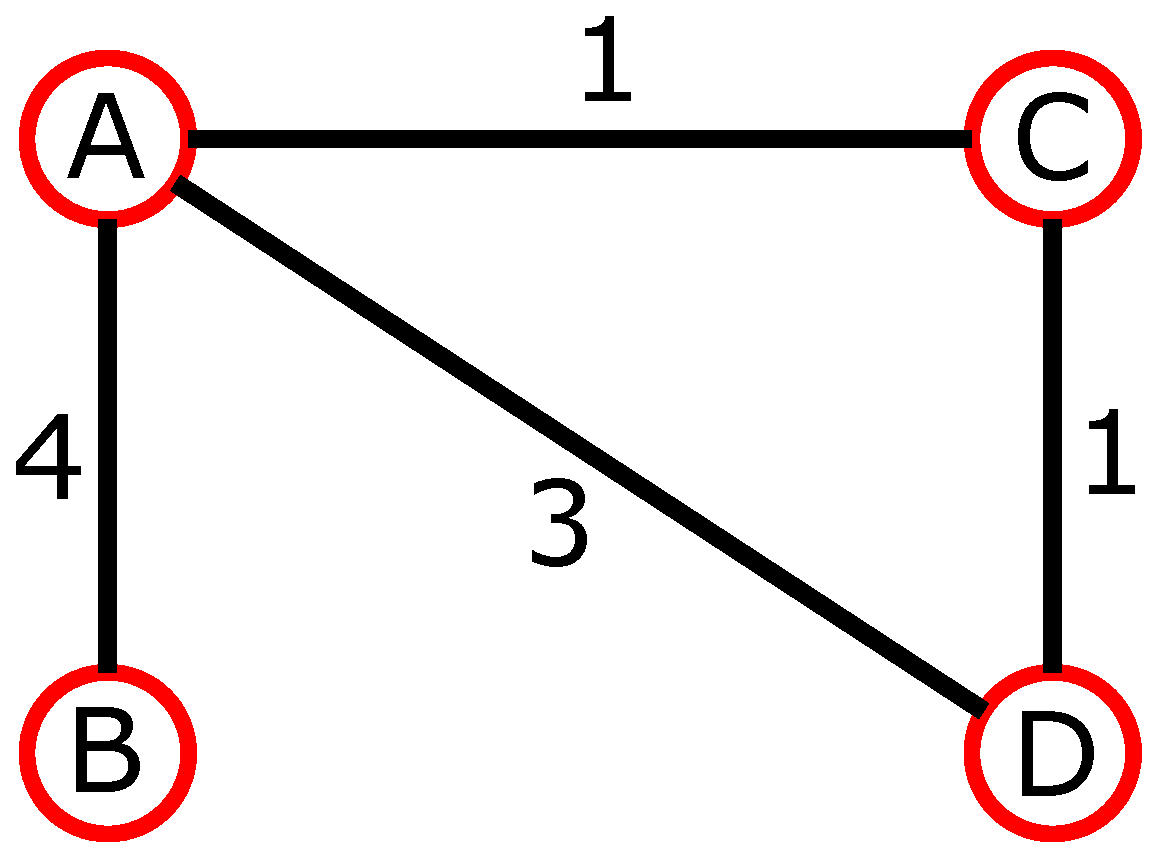
\includegraphics[width=50mm]{DV.eps}
\end{figure}
Q3) In the following network, assume node A wishes to broadcast a packet of size 5Kbytes to all other nodes. How many bytes, in total, would be transmitted over all the network links if
\begin{enumerate}[label=\alph*-]
\item
uncontrolled flooding
\item
controlled flooding using the reverse path forwarding approach
\item
minimum-spanning tree with center-based approach
\end{enumerate}
is used? All the link costs are assumed to be 1.

(In part c-, also fully explain the steps of attaining such spanning tree.)
\begin{figure}[htbp]
\centering
\includegraphics[width=120mm]{broadcast.pdf}
\end{figure}

Q4) In the following network (next page), a group of nodes, denoted by red, decide to join a multicast group and all other nodes (denoted by black) are inactive for the multicast session. The source node is attached to router A.
\begin{enumerate}[label=\alph*-]
\item
Which routers have at least one multicast node attached to?
\item
In a \textit{Multicast routing approach using a source-based tree}, If the subgraph whose links are denoted by blue is the multicast forwarding tree, which router(s) have no multicast node attached to but included in the tree?
\item
If pruning is supported, single out the routers that will send a prune message to their upstream router (also include your reasons).
\item
(Optional) After pruning is done and irrelevent routers were dropped out from the network, which tree links will be declared as useless and detached from the tree?
\end{enumerate}
\begin{figure}[htbp]
\centering
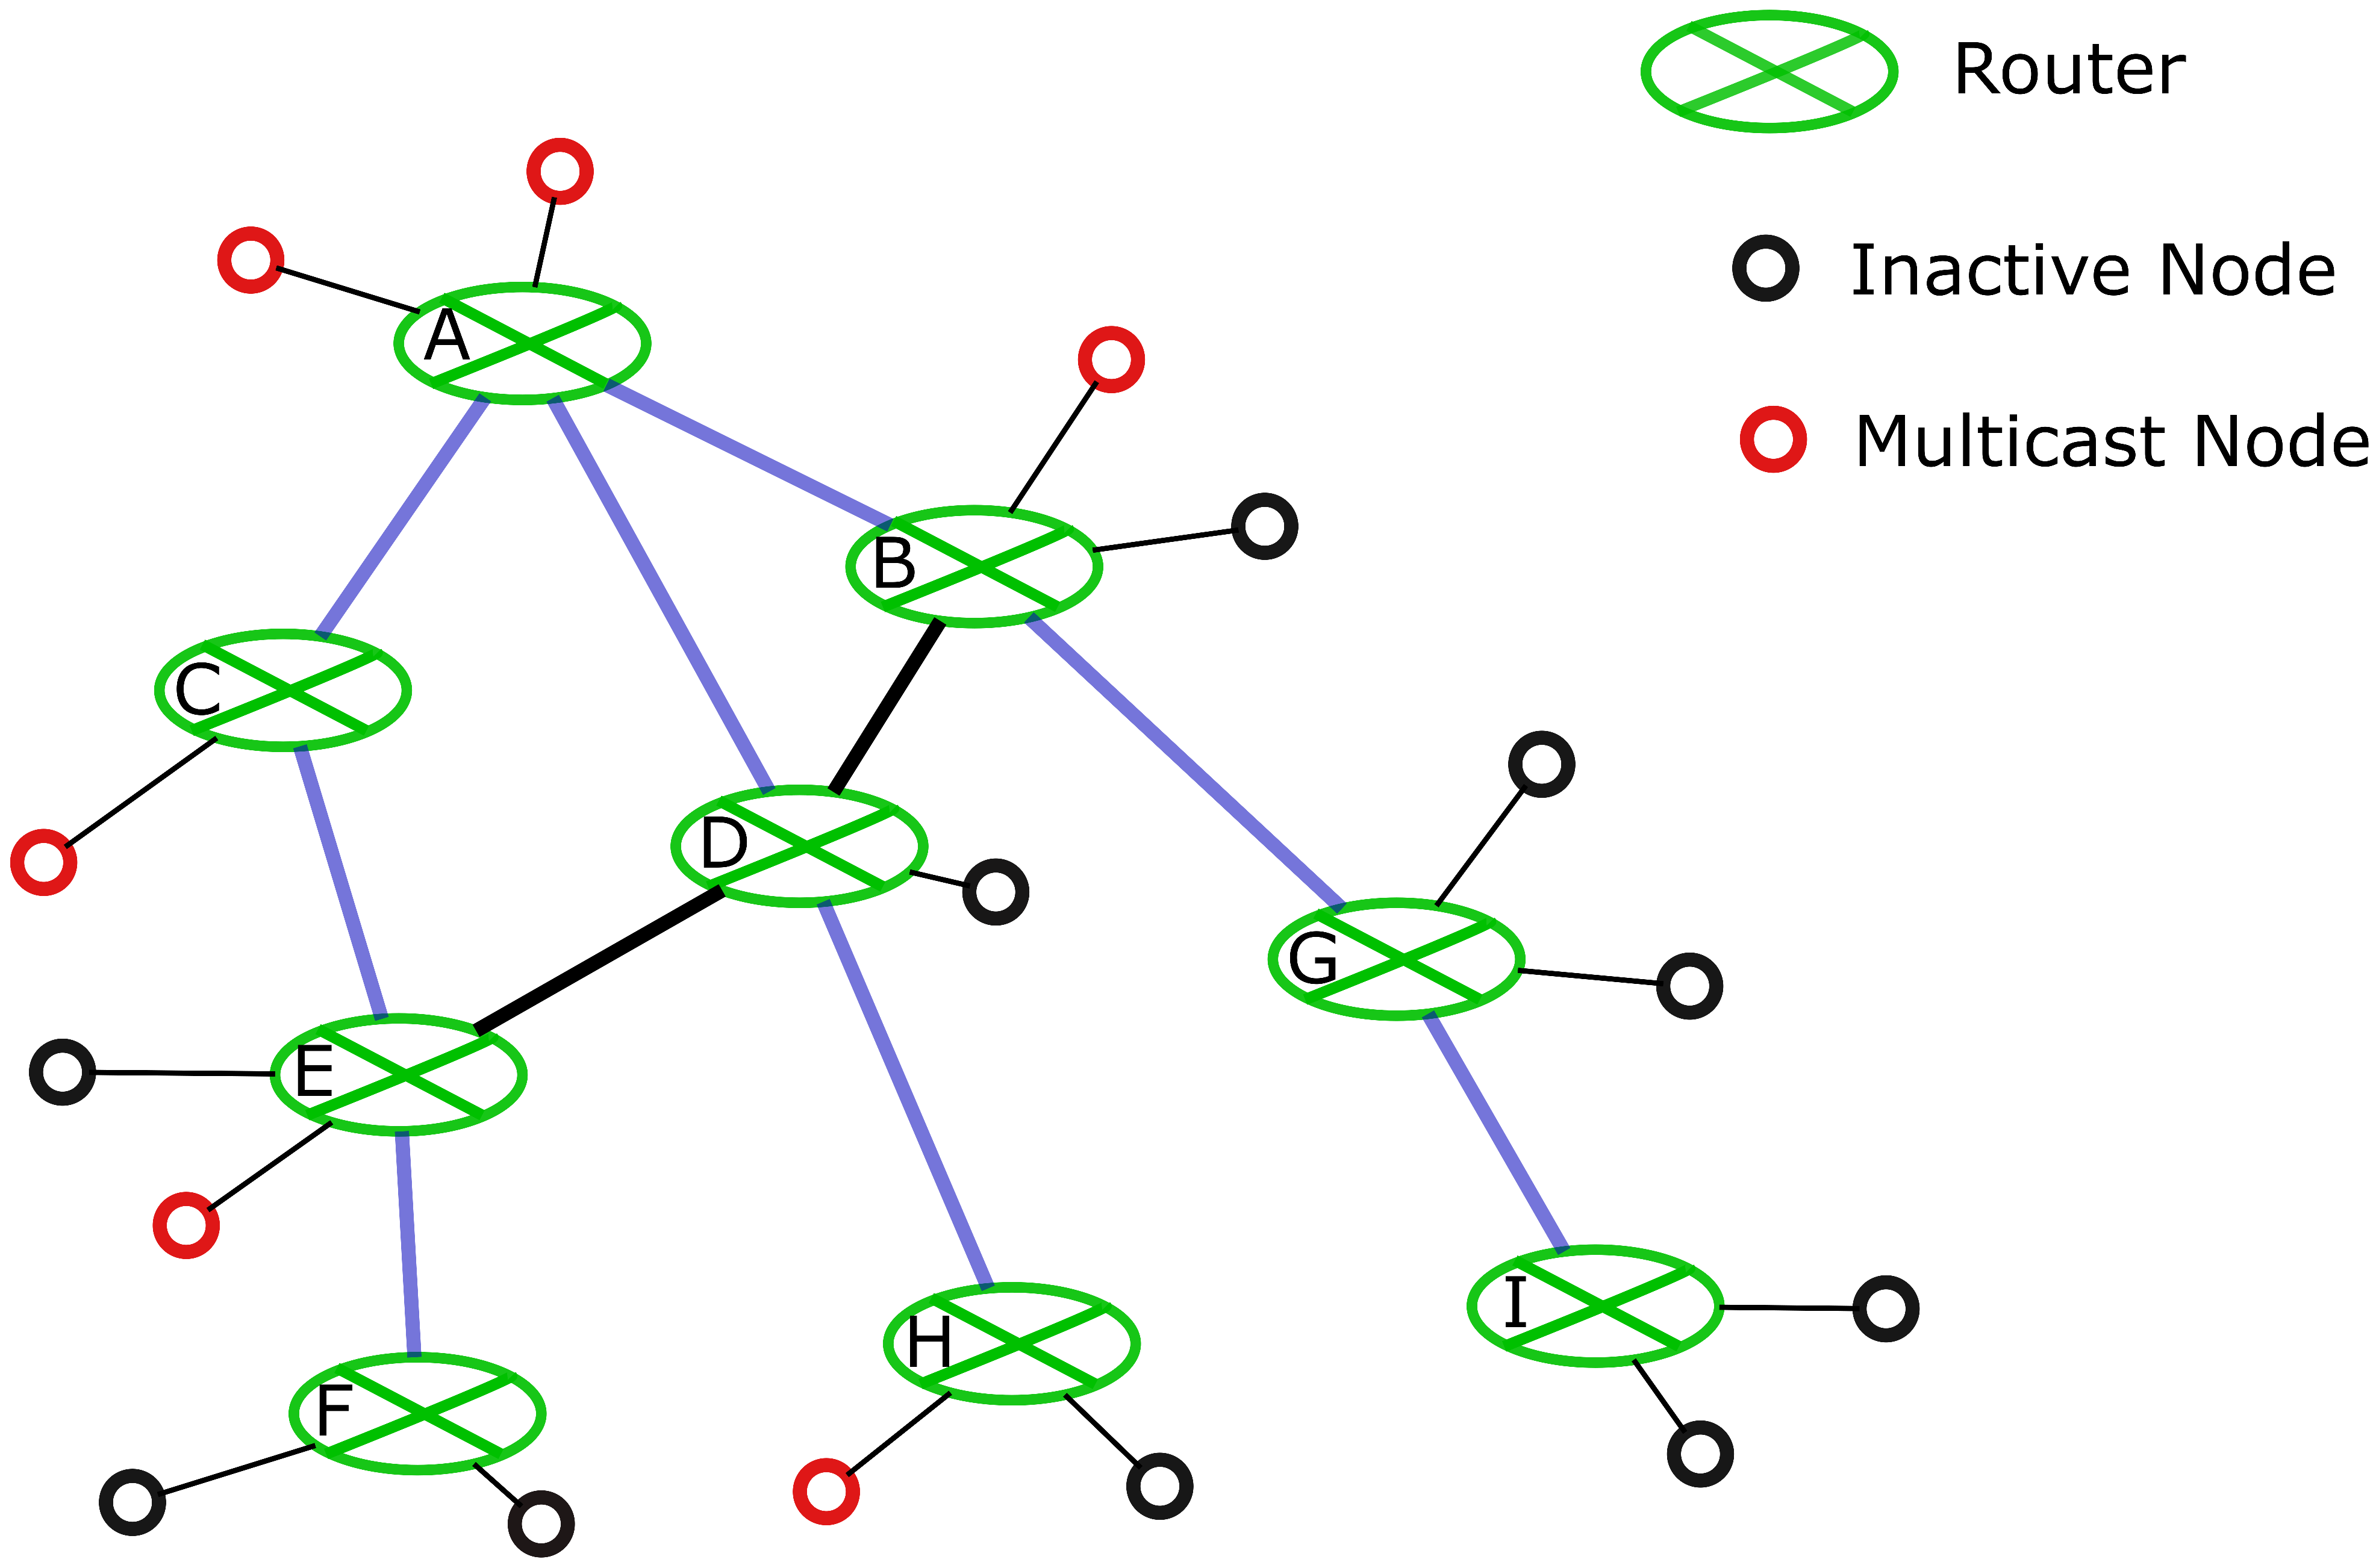
\includegraphics[width=140mm]{multicast.eps}
\end{figure}

\end{document}